\section{Tucker Polynomial Models}
\label{sec:model}

\subsection{Tucker as a Linear Core Map}
\label{sec:problem}

Let $\cY \in \R^{I_1 \times \cdots \times I_N}$ denote the measured tensor and
let $\Omega \in \{0,1\}^{I_1 \times \cdots \times I_N}$ be the observation
mask. A Tucker tensor is
\begin{equation}
  \cS =
  \tucker{\cX}{\bA^{(1)},\ldots,\bA^{(N)}} ,
  \label{eq:latent_tucker}
\end{equation}
where $\cX \in \R^{R_1 \times \cdots \times R_N}$ is the core and
$\bA^{(n)} \in \R^{I_n \times R_n}$ are mode factors. Entrywise,
\begin{equation}
  S_{\mathbf{i}}
  =
  \sum_{r_1,\ldots,r_N}
  X_{r_1,\ldots,r_N}
  \prod_{n=1}^{N}A^{(n)}_{i_n,r_n}.
  \label{eq:tucker_entry}
\end{equation}
For fixed factors, this is a linear map from the core to the data tensor. The
core controls interactions among the mode coordinates, while the factors map
those coordinates to the observed dimensions.

\subsection{Tucker Polynomial Model}

We extend the linear core map by allowing polynomial interactions among core
entries. Throughout, $P$ denotes the maximum polynomial degree and $p$ indexes
a degree. For $p\ge 1$, define a $p$-fold Tucker term by
\begin{equation}
\begin{aligned}
  [\mathcal{T}_p(\cX)]_{\mathbf{i}}
  ={}&
  \sum_{\mathbf{r}^{(1)},\ldots,\mathbf{r}^{(p)}}
  \prod_{\ell=1}^{p}X_{\mathbf{r}^{(\ell)}}
  \prod_{n=1}^{N}
  \mathcal{A}^{(n,p)}_{
  i_n,r_n^{(1)},\ldots,r_n^{(p)}} .
\end{aligned}
  \label{eq:pfold_tucker}
\end{equation}
Here $\ell=1,\ldots,p$ indexes the core copies and
$\mathcal{A}^{(n,p)}$ is the order-$p$ mode map for mode $n$. When $p=1$,
choosing $\mathcal{A}^{(n,1)}=\bA^{(n)}$ recovers standard Tucker. For
$p\ge2$, the term is a degree-$p$ polynomial in the core entries.
Figure~\ref{fig:pfold-tucker-network} visualizes these contractions for $N=3$.
The degree label on $\mathcal A^{(n,p)}$ is omitted inside the nodes to keep the
diagram readable.

\begin{figure}[!t]
  \centering
  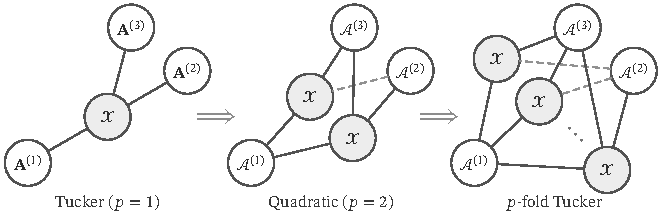
\includegraphics[width=\columnwidth]{figures/pfold_tucker_network.pdf}
  \caption{Tensor-network view of the $p$-fold Tucker term in
  \eqref{eq:pfold_tucker} for $N=3$. Starting from Tucker, the quadratic and
  general $p$-fold terms connect two or $p$ copies of the core to the same
  three mode maps. Dashed edges and the ellipsis reduce visual clutter.}
  \label{fig:pfold-tucker-network}
\end{figure}

Summing several orders gives the Tucker polynomial
\begin{equation}
  \widehat{\cY}
  =
  \beta_0\mathbf{1}
  +
  \sum_{p=1}^{P}\beta_p\mathcal{T}_p(\cX).
  \label{eq:tucker_polynomial}
\end{equation}

The general model assigns a separate mode map to every order. It provides a
direct polynomial extension of Tucker, but its parameter count grows quickly
with $p$. It is the general starting model; the next subsection derives the
compact form used for estimation.

\subsection{Shared Factors and NTD-PL}

We share the original Tucker factors across polynomial orders by setting
\begin{equation}
  \mathcal{A}^{(n,p)}_{
  i_n,r_n^{(1)},\ldots,r_n^{(p)}}
  =
  \prod_{\ell=1}^{p}A^{(n)}_{i_n,r_n^{(\ell)}}.
  \label{eq:shared_pfold_factors}
\end{equation}
Substituting this relation into \eqref{eq:pfold_tucker} gives
\begin{equation}
  \mathcal{T}_p(\cX)=\cS^{\od p}.
  \label{eq:shared_pfold_equivalence}
\end{equation}
The shared-factor Tucker polynomial is therefore
\begin{equation}
  \widehat{\cY}
  =
  f_{\bbeta}(\cS)
  =
  \sum_{p=0}^{P} \beta_p \cS^{\od p},
  \label{eq:polynomial_linked_tucker}
\end{equation}
which is NTD-PL. The explicit expansion and its ordinary Tucker representation are
given in the supplementary material.

Equation~\eqref{eq:polynomial_linked_tucker} also gives the nonlinear
measurement interpretation
\begin{equation}
  Y_{\mathbf{i}}=f_{\bbeta}(S_{\mathbf{i}})+\varepsilon_{\mathbf{i}},
  \qquad
  \mathbf{i}=(i_1,\ldots,i_N),
  \label{eq:measurement_model}
\end{equation}
where $\varepsilon_{\mathbf{i}}$ denotes measurement noise. Thus NTD-PL is both
a compact Tucker polynomial and a low-rank Tucker tensor followed by a shared
entrywise response. Sharing the factors removes the separate high-order mode
maps; compared with Tucker, the only additional trainable variables are the
$P+1$ response coefficients.

The data determine the combined prediction $f_{\bbeta}(\cS)$. Without external
calibration constraints, we do not claim that the fitted $\cS$ and response
recover a unique physical measurement process.

\subsection{Other Response Bases}

The estimator is not limited to powers. A finite set of scalar basis functions
gives
\begin{equation}
  \widehat{\cY}
  =
  f_{\bbeta}(\cS)
  =
  \sum_{j=0}^{J} \beta_j \psi_j(\cS),
  \label{eq:finite_response_tucker}
\end{equation}
where $J+1$ is the number of basis functions and $\psi_j(\cS)$ applies
$\psi_j$ entrywise. Standard Tucker is recovered
when the fitted response is the identity. Possible alternatives include
conditioned polynomial bases, radial basis functions, and splines. These
choices retain the same Tucker representation and estimation objective. The
$p$-fold Tucker derivation applies to the power basis, which is the main
model used in this paper.

\subsection{Masked Recovery Objective}

The same formulation covers reconstruction and completion. We estimate the
core, factors, and response coefficients by minimizing
\begin{equation}
  \min_{\cX,\{\bA^{(n)}\},\bbeta}
  \frac{1}{2|\Omega|}
  \norm{\Omega \od \left(\cY - f_{\bbeta}(\cS)\right)}_F^2
  +
  \mathcal{R}(\cX,\{\bA^{(n)}\},\bbeta),
  \label{eq:masked_objective_model}
\end{equation}
where $\mathcal{R}$ contains regularization terms for the Tucker parameters and
the response coefficients. For reconstruction, $\Omega$ contains all entries.
For completion, $\Omega$ selects the entries used for fitting, and the remaining
entries are used for evaluation.
